\documentclass[sigconf]{acmart}
% Cleaning
\pagestyle{fancy} % removes running headers
\settopmatter{printacmref=false} % Removes citation information below abstract
\renewcommand\footnotetextcopyrightpermission[1]{} % removes footnote with conference information in first column
\pagestyle{plain} % removes running headers
\fancyhead{}
\settopmatter{printacmref=false, printfolios=false}
% Copyright
\setcopyright{none}
% \setcopyright{acmcopyright}
% \setcopyright{acmlicensed}
% \setcopyright{rightsretained}
% \setcopyright{usgov}
% \setcopyright{usgovmixed}
% \setcopyright{cagov}
% \setcopyright{cagovmixed}
\settopmatter{printacmref=false} % Removes citation information below abstract
\acmDOI{}
\acmConference[CSC503/SENG474]{CSC503 \texttimes{} SENG474: Data Mining}{Fall 2026}{University of Victoria}

\usepackage{booktabs} % For formal tables
\usepackage{url}
\usepackage{algorithm}
\usepackage[noend]{algpseudocode}
\usepackage{tikz}
\usetikzlibrary{arrows.meta,positioning,fit}


\setlength{\parskip}{0pt}
\setlength{\parsep}{0pt}
\setlength{\headsep}{0pt}
\setlength{\topskip}{0pt}
\setlength{\topmargin}{0pt}
\setlength{\topsep}{0pt}
\setlength{\partopsep}{0pt}
%\linespread{0.95}
\usepackage{mdwlist}
\usepackage{amsmath}

\begin{document}
\title{Geospatial Foundation Model Embedding-Augmented Attention-U-Net for Next-Day Wildfire Spread Prediction}

\author{Sebastian Brubaker}
\affiliation{\institution{University of Victoria}\city{Victoria}\state{British Columbia}\country{Canada}}
\email{sebastian.brubaker@gmail.com}

\author{Armaan Binpal}
\affiliation{\institution{University of Victoria}\city{Victoria}\state{British Columbia}\country{Canada}}
\email{armaanbinpal1@gmail.com}

\author{James Kim}
\affiliation{\institution{University of Victoria}\city{Victoria}\state{British Columbia}\country{Canada}}
\email{jknhjk03@uvic.ca}

\author{Bowen Zhang}
\affiliation{\institution{University of Victoria}\city{Victoria}\state{British Columbia}\country{Canada}}
\email{7pixels.v@gmail.com}


\begin{abstract}
We specify a geospatial foundation-model-augmented Attention U-Net for pixel-wise prediction of the next 
day's wildfire mask. Twelve conventional channels from the Next Day Wildfire Spread dataset are concatenated with 
spatially aggregated 64-dimensional annual AlphaEarth embeddings to the dataset's 1-km grid, yielding a 
$76\times64\times64$ input. To retain an actual observed embedding, each 1-km cell is 
represented by the exact cosine medoid of its valid fine-resolution embeddings. The annual embedding is selected from 
the preceding calendar year to prevent data leakage. We describe the input-output mapping, preprocessing, 
model architecture, and a training and inference procedure. 
Project repository: https://github.com/CSC503-Wildfire-Team/Wildfire-Prediction-DL
\end{abstract}

\keywords{asdkjhf, askdjhf}
\maketitle

\section{Introduction}
Next-day wildfire spread prediction is framed as segmentation--dense image classification: given the observed fire state and 
environmental conditions at day $t$, estimate the fire mask at $t+1$. The Next Day Wildfire Spread (NDWS) dataset 
represents U.S. fire events from 2012--2020 and provides daily fire masks and aligned environmental predictors 
at a 1-km spatial resolution; each $64\times64$ patch represents a $64\,\mathrm{km}\times64\,\mathrm{km}$ region 
\cite{huot}. The NDWS describes drivers using physical quantities, in contrast, AlphaEarth Foundations (AEF) produces 
general-purpose geospatial representations by learning from multiple Earth-observation sources and releases annual 
64-dimensional embedding layers at approximately 10-m spatial resolution \cite{brown}.

We propose augmenting the NDWS feature stack with AEF embeddings, yielding a wildfire predictor suitable for an 
Attention U-Net architecture. The methodological contribution is a temporally constrained, spatially aggregated 
feature-fusion pipeline that leverages the spatially selective skip connections of the wildfire Attention U-Net 
proposed by Almakrami et al. \cite{almakrami} to transfer annual AEF context to the daily 1-km prediction grid of NDWS.


\section{Problem Definition}
For a sample at date $t$, let $\mathbf{X}_t\in\mathbb{R}^{12\times64\times64}$ be the conventional input and 
$\mathbf{Y}_{t+1}\in\{0,1\}^{64\times64}$ the next-day fire mask. The 12 channels are 11 drivers (elevation; wind 
direction/speed; minimum/maximum temperature; humidity; precipitation; PDSI; NDVI; population density; ERC) plus 
the day-$t$ fire mask \cite{huot}. Let $\mathbf{E}_t\in\mathbb{R}^{64\times64\times64}$ be the AEF tensor aligned to 
the same grid. The proposed predictor may be expressed as a function
\begin{equation}
 f_\theta:\mathbb{R}^{76\times64\times64}\rightarrow[0,1]^{64\times64},\qquad
 f_\theta(\mathbf{Z}_t) = \widehat{\mathbf{Y}}_{t+1},\quad
 \mathbf{Z}_t=\mathbf{X}_t\mathbin{\Vert}_{C}\mathbf{E}_t,
 \label{eq:problem}
\end{equation}
where $\Vert_C$ denotes concatenation along the channel axis and $\theta$ denotes the set of trainable parameters.


\section{Proposed Method}
\subsection{Temporal and Spatial Embedding Alignment}
AEF represents spatial and temporal context in a 64-dimensional embedding and provides annual layers beginning in 2017 
\cite{brown}. For an event in calendar year $y$, the annual layer indexed $y-1$ is used to prevent data leakage. 
Because the released archive begins in 2017, this preceding-year join is available for NDWS samples from 2018--2020; 
earlier samples have no preceding layer and are therefore excluded.

For each 1-km NDWS cell $g$, let $V_g=\{\mathbf{v}_{g,1},\ldots,\mathbf{v}_{g,n_g}\}$ be the valid 64-D AEF pixel 
vectors spatially assigned to that cell after geospatial alignment ($|V_g| \approx 10,000$). Normalize each vector, 
$\bar{\mathbf{v}}_{g,i}=\mathbf{v}_{g,i}/\|\mathbf{v}_{g,i}\|_2$, and select the exact cosine medoid as:
\begin{equation}
 i_g^* = \underset{{i\in\{1,\ldots,n_g\}}}{\text{argmax}}
 \sum_{j=1}^{n_g}\bar{\mathbf{v}}_{g,i}^{\top}\bar{\mathbf{v}}_{g,j},\qquad
 \mathbf{e}_g = \bar{\mathbf{v}}_{g,i_g^*}.
 \label{eq:medoid}
\end{equation}
Observe, $L_2$ normalizing yields unit vectors, making the inner product equivelent to cosine similarity. Additionally, 
note that the medoid is an observed AEF vector rather than a component-wise aggregate. Invalid pixels are excluded. 
Note, one vector per cell loses sub-kilometre heterogeneity and may suppress minority patterns.

\subsection{Preprocessing and Channel Fusion}
The medoids are composed to form $\mathbf E_t$ on the NDWS grid. Each NDWS feature channel is 
standardized, $\widetilde X_{t,c}=(X_{t,c}-\mu_c)/\sigma_c$, following \cite{almakrami}. Concatenate 
$\widetilde{\mathbf X}_t$ with the 64 medoid channels to obtain $\mathbf Z_t$ as described in equation \eqref{eq:problem}.

\begin{figure}[t]
\centering
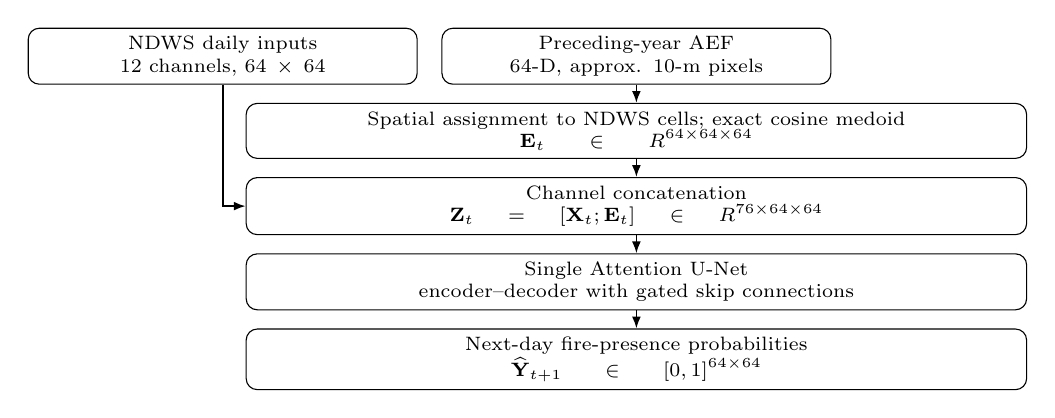
\begin{tikzpicture}[
  n/.style={draw,rounded corners,align=center,font=\scriptsize,inner sep=3pt,minimum height=6mm,text width=0.80\columnwidth},
  s/.style={draw,rounded corners,align=center,font=\scriptsize,inner sep=3pt,minimum height=7mm,text width=0.39\columnwidth},
  a/.style={-{Latex[length=1.5mm]},semithick},
  node distance=2.3mm and 3mm]
  \node[s] (x) {NDWS daily inputs\\12 channels, $64\times64$};
  \node[s,right=of x] (ae) {Preceding-year AEF\\64-D, approx. 10-m pixels};
  \node[n,below=of ae] (med) {Spatial assignment to NDWS cells; exact cosine medoid\\$\mathbf E_t\in\mathbb R^{64\times64\times64}$};
  \node[n,below=of med] (cat) {Channel concatenation\\$\mathbf Z_t=[\mathbf X_t;\mathbf E_t]\in\mathbb R^{76\times64\times64}$};
  \node[n,below=of cat] (net) {Single Attention U-Net\\encoder--decoder with gated skip connections};
  \node[n,below=of net] (out) {Next-day fire-presence probabilities\\$\widehat{\mathbf Y}_{t+1}\in[0,1]^{64\times64}$};
  \draw[a] (x.south) |- (cat.west);
  \draw[a] (ae.south)--(med.north);
  \draw[a] (med.south)--(cat.north);
  \draw[a] (cat.south)--(net.north);
  \draw[a] (net.south)--(out.north);
\end{tikzpicture}
\caption{Feature construction and single-stream prediction.}
\label{fig:pipeline}
\end{figure}

\subsection{Attention U-Net}
Adapting the wildfire Attention U-Net proposed by Almakrami et al. \cite{almakrami}, the input layer is modified to receive 76
channels while the remaining architecture is left unchanged. Four encoder levels each use double convolutions, consisting of
$3 \times 3$ convolutions, batch normalizations, and ReLUs, followed by $2\times2$ max pooling; a two-convolution, 1024-filter
bridge captures coarse context. The decoder upsamples and fuses attention-gated skip connections.

The feature map at level $l \in \{1, 2, 3, 4\}$ of the encoding path $\mathbf{F}^{enc}_{l}$ is given by:
\begin{equation}
\mathbf{C}^{enc}_{l} = \operatorname{ReLU}\left(
  \operatorname{BN}\left(
    \mathbf{W}_{l,2}^{enc} * \operatorname{ReLU}\left(
      \operatorname{BN}\left(
        \mathbf{W}_{l,1}^{enc} * \mathbf{F}^{enc}_{l-1}
      \right)
    \right)
  \right)
\right)
\label{eq:doubleconv}
\end{equation}
\begin{equation}
\mathbf{F}^{enc}_{l} =
\operatorname{MaxPool}_{2 \times 2}
\left(\mathbf{C}^{enc}_{l}\right)
\label{eq:maxpool}
\end{equation}
where $\mathbf{C}_{l}^{enc}$ is the convolved feature map, $\mathbf{W}_{l,1}^{enc}$ and $\mathbf{W}_{l,2}^{enc}$ are learnable parameters, 
and $*$ denotes convolution, $\operatorname{BN}$ denotes batch normalization, $\operatorname{ReLU}$ denotes the rectified linear 
unit activation.

At each corresponding decoder level $l$, an additive attention gate filters the corresponding encoder feature map using the preceding decoder feature map as a gating signal. The attention coefficients are computed as:
\begin{equation}
\mathbf{A}_{l} =
\sigma\left(
\mathbf{W}_{l,3}^{\top [att]} *
\operatorname{ReLU}\left(
  \mathbf{W}_{l,2}^{att} * \mathbf{F}^{dec}_{l+1}
  +
  \mathbf{W}_{l,1}^{att} * \mathbf{C}^{enc}_{l}
  +
  \mathbf{b}_{l}
\right)
\right)
\label{eq:attention}
\end{equation}
where $\mathbf{W}_{l,1}^{att}$ and $\mathbf{W}_{l,2}^{att}$ are learnable parameters, $\mathbf{W}_{l,3}^{\top [att]}$ projects the combined representation to a single-channel attention score, $\mathbf{b}_{l}$ is a learnable bias, and $\sigma$ denotes the sigmoid function. The gated encoder features are then obtained by:
\begin{equation}
\hat{\mathbf{F}}^{enc}_{l} =
\mathbf{A}_{l} \odot \mathbf{C}^{enc}_{l}
\label{eq:gatedfeatures}
\end{equation}
where $\odot$ denotes element-wise multiplication.

The gated features are concatenated with the upsampled decoder features, and passed through a double-convolution block:
\begin{equation}
\mathbf{F}^{dec}_{l} =
\operatorname{ReLU}\left(
  \operatorname{BN}\left(
    \mathbf{W}_{l,2}^{dec} * \operatorname{ReLU}\left(
      \operatorname{BN}\left(
        \mathbf{W}_{l,1}^{dec} *
          \hat{\mathbf{F}}^{enc}_{l}
          \Vert_C
          \operatorname{UpConv}_{2 \times 2}
          (\mathbf{F}^{dec}_{l+1})
      \right)
    \right)
  \right)
\right)
\label{eq:decoding}
\end{equation}

Finally, the output is given by
\begin{equation}
\hat{\mathbf{Y}} =
\sigma\left(
\mathbf{W}^{out}_1 * \mathbf{F}^{dec}_{1}
\right)
\label{eq:prediction}
\end{equation}
where $\mathbf{W}^{out}_1$ is a learnable parameter and $*$ is a $1 \times 1$ convolution. 

\bibliographystyle{ACM-Reference-Format}
\bibliography{bibliography}

\end{document}
